%% 
%% Copyright 2007, 2008, 2009 Elsevier Ltd
%% 
%% This file is part of the 'Elsarticle Bundle'.
%% ---------------------------------------------
%% 
%% It may be distributed under the conditions of the LaTeX Project Public
%% License, either version 1.2 of this license or (at your option) any
%% later version.  The latest version of this license is in
%%    http://www.latex-project.org/lppl.txt
%% and version 1.2 or later is part of all distributions of LaTeX
%% version 1999/12/01 or later.
%% 
%% The list of all files belonging to the 'Elsarticle Bundle' is
%% given in the file `manifest.txt'.
%% 

%% Template article for Elsevier's document class `elsarticle'
%% with numbered style bibliographic references
%% SP 2008/03/01

\documentclass[preprint,12pt]{elsarticle}

%% Use the option review to obtain double line spacing
%% \documentclass[authoryear,preprint,review,12pt]{elsarticle}

%% Use the options 1p,twocolumn; 3p; 3p,twocolumn; 5p; or 5p,twocolumn
%% for a journal layout:
%% \documentclass[final,1p,times]{elsarticle}
%% \documentclass[final,1p,times,twocolumn]{elsarticle}
%% \documentclass[final,3p,times]{elsarticle}
%% \documentclass[final,3p,times,twocolumn]{elsarticle}
%% \documentclass[final,5p,times]{elsarticle}
%% \documentclass[final,5p,times,twocolumn]{elsarticle}

%% For including figures, graphicx.sty has been loaded in
%% elsarticle.cls. If you prefer to use the old commands
%% please give \usepackage{epsfig}

%% The amssymb package provides various useful mathematical symbols
\usepackage{amssymb}
%% The amsthm package provides extended theorem environments
%% \usepackage{amsthm}

%% The lineno packages adds line numbers. Start line numbering with
%% \begin{linenumbers}, end it with \end{linenumbers}. Or switch it on
%% for the whole article with \linenumbers.
%% \usepackage{lineno}

\journal{Decision Support Systems}

\begin{document}

\begin{frontmatter}

%% Title, authors and addresses

%% use the tnoteref command within \title for footnotes;
%% use the tnotetext command for theassociated footnote;
%% use the fnref command within \author or \address for footnotes;
%% use the fntext command for theassociated footnote;
%% use the corref command within \author for corresponding author footnotes;
%% use the cortext command for theassociated footnote;
%% use the ead command for the email address,
%% and the form \ead[url] for the home page:
%% \title{Title\tnoteref{label1}}
%% \tnotetext[label1]{}
%% \author{Name\corref{cor1}\fnref{label2}}
%% \ead{email address}
%% \ead[url]{home page}
%% \fntext[label2]{}
%% \cortext[cor1]{}
%% \address{Address\fnref{label3}}
%% \fntext[label3]{}

\title{Distributed Decision Making for Dynamic Formation of Web Services Communities}

%% use optional labels to link authors explicitly to addresses:
%% \author[label1,label2]{}
%% \address[label1]{}
%% \address[label2]{}

\author{}

\address{}

\begin{abstract}
Web services are loosely-coupled business applications willing to cooperate in distributed settings within different groups called communities. Communities aim to provide web services with better visibility, efficiency, market share and total payoff. A number of mechanisms and models have been recently proposed to aggregate web
services and make them cooperate within their communities. However, existing community models mostly focus on short term goals. Moreover, these models generally suffer from high computational complexity, which makes decision making about community formation in real-time extremely hard, time consuming, and even impossible in some complex cases. In this paper, we propose a strategic distributed decision making mechanism called DDM that regulates web service agents' decision making process, which is about deciding with whom to cooperate. This model first generates a trained set of data based on information obtained from large number of web services regarding their single and cooperative utilities as well as environmental parameters such as demand, service quality, etc. The decision making mechanism implements a decision tree of possible viable strategies and their long-term expected utility gain.
%Utilizing the training model, the decision making mechanism implements a decision tree with an estimation of long-term utility gain for the web services. Communities can used the trained model and instantly choose best-response strategies considering their long-term gain. 
Our model helps 1) communities of web services efficiently find the appropriate web service to invite as new member; and 2) single web services find best communities to join. After being trained, web services get to compute expectations as utilities they would gain if cooperating with communities of different characteristics. In contrast, communities can consider the training into account and analyze the characteristics of different individual web services and make prudent decisions when inviting a web service to join or accepting a join inquiry initiated initiated by a web service. In general, DDM equips web services with efficient methods of foreseeing how their choices of actions would impact their short-term and long-term goals, therefore opting for better decisions. We performed experiments using real data from 142 users on 4,532 web services on 64 different time slots. The experimental results, show that our algorithms provide web services and community owners, in real-world-like environments, with applicable and near-perfect decision making mechanisms.
\end{abstract}

\begin{keyword}
Web services\sep Community of services\sep Distributed Decision Making
%% keywords here, in the form: keyword \sep keyword

%% PACS codes here, in the form: \PACS code \sep code

%% MSC codes here, in the form: \MSC code \sep code
%% or \MSC[2008] code \sep code (2000 is the default)

\end{keyword}

\end{frontmatter}

%% \linenumbers

%% main text
\section{Introduction}

\IEEEPARstart{O}{ver} the past years, online services have become an important part of many scalable business applications. The increasing reliance on online service providers has significantly influenced the way web services are engineered. Therefore, given the dynamic and unpredictable nature of the Internet, delivering high quality services is still a critical and challenging issue. One practical solution towards delivering high quality services is utilizing intelligent decision making agents. These agents aim at maximizing their gain by exploring the best ways to provide services that satisfy end users\cite{Zeng:2003:QDW:775152.775211, 10.1109/ARES.2008.7, journals/tsc/ZhengZYB13, Demirkan2013412}. However, agent-based web services are functionally limited in the sense that they cannot handle a large number of requests at the same time without compromising the quality of service provided. Recent developments have attempted to shift web services from passive models, consisting of individual components, to models made up of autonomous and group-based components that share common goals. In group-based models, interaction, composition, and cooperation are the key challenges \cite{ICWS2011-1, SCC2011-1, journals/mags/BaldoniBM10, journals/jcss/CasadoYT13} that directly impact the group's overall performance in achieving common goals. To that end, we see the emergence of web service \emph{communities}, which consist of services with similar functionalities but distinct nonfunctional properties \cite{Zeng:2003:QDW:775152.775211, Paik:2005:TSS:2229263.2230038, Medjahed05adynamic, 10.1109/ARES.2008.7}. A \emph{community} of web services runs continuous performance assessment functions that regulate web services' interactions and manage their composition and cooperation.

The advantages of community of web services are that the community facilitates the discovery of web services and provides better quality of service compared to passive models with individual components. Communities act as abstract web services, communicating with external entities via the same standard protocols that a normal web service employs. But, they regulate the service process via sophisticated internal communication protocols, thereby providing services based on the combined work of a number of web services. The downside to communities is the complexity of management involved in finding and inviting individual web services and managing the overall quality of the combined work of several web services.
% because although they have similar functionality, they have different attitudes. 
When interacting with communities of web services, users send their requests to the coordinators of the community, which play the role of community representative or access point. The community coordinator is responsible of receiving tasks and delivering services. Moreover, as community representative, it verifies the credentials of new web services before accepting them into the community and kicks web services that could harm the value of the community. 

\textbf{Challenge and Problem Statement.} In recent work, communities of web services have been proposed in order to facilitate discovery of web services, improve the Quality of Service (QoS), and help individual services find better market share and opportunities. However, there is a twofold challenge that yet to be addressed. The first part is community development, which involves finding the right web services for the community, satisfying the objectives of all the web services and community coordinators involved within the community; and the second part is from the individual web service's side because each web service aims to join the community that would guarantee the best outcome. The advocated solutions \cite{conf/webist/MaamarLBTS07, 10.1109/ARES.2008.7, journals/soca/XuYLZB11, 10.1109/TSC.2012.12, managing-hela-jalel, DBLP:conf/IEEEscc/KhosravifarABT11, DBLP:conf/IEEEscc/LimTMB12} have attempted to address these research problems. These research problems are reflected by the two challenge parts: 
\begin{enumerate}
	\item The solutions consider the architecture of centralized management for communities where most of the decisions are made by the centralized coordinator. The problem is that in real world scenarios, decisions made by independent service providers are highly distributed.
	\item The solutions either propose complex algorithms \cite{DBLP:conf/IEEEscc/LimTMB12, 10.1109/TSC.2012.12, 10.1109/TSC.2014.2312940} to find the optimal strategy to follow, or oversimplify the problem by eliminating important parameters and using approximation techniques to make the algorithms tractable \cite{10.1109/TSC.2012.12}.
\end{enumerate}
These approximation methods sometimes negatively influence the outcome because simplifying the constraints may cause important aspects of the problem to be ignored. 

For example, instead of calculating the gain distribution using the complex shapely-value method, \cite{10.1109/TSC.2012.12} proposes a simple egalitarian way of distributing gain, which completely ignores the gain generated from collaborative work of sub-communities. Other categories of related work exist that do not focus on all the parties involved within the community \cite{DBLP:conf/IEEEscc/KhosravifarABT11}. 
%And some other work which do not focus on rationality on web services or communities involved [refrences]. 
In \cite{journal-community-formation} we proposed a cooperative game theory based model for aggregating web services in communities. A centralized decision maker in communities based on a complete knowledge of available web service quality metrics and performance, has been used to form optimal and stable communities that maximize individual and group income. However, centrality and complete information are strong assumptions, which are not very compatible with real business scenarios.

\textbf{Contributions.} In this paper, we introduce DDM, a Distributed Decision Making model for  community formation that regulates web service agents’ decision making process in terms of cooperating and deciding which group to join and which service to invite for joining. The decision model in extracted from a data model in the form of information obtained from a large number of web services regarding their single and cooperative utilities as well as environmental parameters such as demand, service quality, etc. The generated decision tree improves agents' understanding of the environment and how to select actions that lead towards maximizing their utilities. The advantage of this approach is that the tree is created from the past data and reflects comprehensive vision about agents' attitude of action selection. However, the tree is subject to get continuously modified to adapt with environmental changes.
%The training model deploys a logistic regression algorithm to build a hypothesis function that can thoroughly address the aforementioned research problems. 
The decision model provides web services with enough information which helps those services to efficiently decide and predict the outcome of their different possible collaborations. This model works in a distributed manner in which services are self-sufficient in decision making process and do not rely on a centralized decision making process. Our findings show that communities of web services can efficiently find the appropriate web service to invite for cooperation as well as allowing a single web service to find the best communities to join. In other words, the web services agents are equipped with a recommender system to suggest beneficial action. Moreover, communities can consider the decision model and analyze the characteristics of different individual web services and make prudent decisions when inviting a web service to join or accepting a join inquiry initiated from a web service. In general, DDM equips web services with efficient methods for foreseeing how their choices will impact their short-term and long-term goals; therefore, opting for best decision available.

To effectively train web services, we used real data set to extract web services' individual characteristics and used them to measure outcomes when they cooperate with one another. The data set has been extracted by real-world QoS evaluation results from 142 users on 4,532 Web services on 64 different time slots. Combining these data based on each web service point of view on different time slots, we acquired 5 different unique features for 4,532 web services. By engineering and extracting these features, we gathered functional and cooperative features for both individual web services and communities in different time slots. We were able to investigate the path a web service might take to achieve the best utility out of effective interaction with others. All paths and the outcomes are labeled to be utilized in the training model. Using cross validation sets, web services are able to compute the optimal hypothesis function (using logistic regression) that can be used to predict outcomes of cooperative work with other individual web services or communities. Our findings show that web services equipped with DDM have by far better outcomes in the form of cooperative service providers than the ones that either do not cooperate or randomly find communities to join. 

\textbf{Organization.} The rest of the paper is organized as follows. In Section 2 we briefly describe the preliminaries and challenging issues. Section 3 discusses the considered parameters and web service community architecture. Section 4 presents our solution model, the way data is trained and the way web services utilize the trained data in their decision making process. Section 5 describes our experiments and results. Section 6 discussed relevant related work. Finally Section 7 concludes the paper and identifies future work.

%- We want to give full distributed control to web services as autonomous agents and distribute the task of community management among all web services and let them decide how to maximize their efficiency and join and create communities.
%- Let agents train and learn long term expectations of each action and group they can join with
%- Web services cannot find the optimal solution in big space problem of many web services
%- Add rationalism and less vague decisions

%Web services provide a set of stateless software functions accessible at a network address over the web. 
%Online autonomous agent-based services are software systems providing a standard way of interoperability among different applications. 

% - The recent developments are shifting web services from passive and individual components to autonomous and group-based components where interactiion, composition, and cooperation are the key challenges. 



%- High demand on online services has created a massive business competition. For example, nowadays users are provided with multiple choices of web services offering local places information such as coffees, venues, and shops nearby a geographic position. It is hard for new web services to find their customers and be visible for end users amongst hundreds or thousands of other available services, even if they provide a high quality of service. Hence, the concept of communities of web services provides them with the chance of joining a platform with an established market share and reputation. However, it is crucial for a community manager to consider many factors when inviting or accepting new members. For example,  this may hurt the community stability.

%- The high competition within the services industry requires applications to use reliable and high quality online service providers. If the user were to check a web site or run an application on her mobile device upon having downtime, or having high response delay or encountering any non-satisfying quality metric, she will instantly remove the application, which is a huge business concern for application providers. For example, if a user installs a ticketing application on her mobile device and the application is not using high quality service providers, the user would instantly uninstall the application, which has an extremely negative impact on the visibility of the application.

%- Most applications cannot independently satisfy users requests and should rely on different online services. The high competition within the services industry requires applications to use reliable and high quality online service providers. 

%Today web services are 

%- softwares rely on third party online service providers 
%- quality of services determines the success of the business 
%- services want to maximise thier utility by cooperating with best possible communities
%- services need to get visible and join market 

% Computer Society journal papers do something a tad strange with the very
% first section heading (almost always called "Introduction"). They place it
% ABOVE the main text! IEEEtran.cls currently does not do this for you.
% However, You can achieve this effect by making LaTeX jump through some
% hoops via something like:
%
%\ifCLASSOPTIONcompsoc
%  \noindent\raisebox{2\baselineskip}[0pt][0pt]%
%  {\parbox{\columnwidth}{\section{Introduction}\label{sec:introduction}%
%  \global\everypar=\everypar}}%
%  \vspace{-1\baselineskip}\vspace{-\parskip}\par
%\else
%  \section{Introduction}\label{sec:introduction}\par
%\fi
%
% Admittedly, this is a hack and may well be fragile, but seems to do the
% trick for me. Note the need to keep any \label that may be used right
% after \section in the above as the hack puts \section within a raised box.



% The very first letter is a 2 line initial drop letter followed
% by the rest of the first word in caps (small caps for compsoc).
%
% form to use if the first word consists of a single letter:
% \IEEEPARstart{A}{demo} file is ....
%
% form to use if you need the single drop letter followed by
% normal text (unknown if ever used by IEEE):
% \IEEEPARstart{A}{}demo file is ....
%
% Some journals put the first two words in caps:
% \IEEEPARstart{T}{his demo} file is ....
%
% Here we have the typical use of a "T" for an initial drop letter
% and "HIS" in caps to complete the first word.
%\IEEEPARstart{T}{his} demo file is intended to serve as a ``starter file''
%for IEEE Computer Society journal papers produced under \LaTeX\ using
%IEEEtran.cls version 1.7 and later.
% You must have at least 2 lines in the paragraph with the drop letter
% (should never be an issue)
%I wish you the best of success.

%\hfill mds

%\hfill January 11, 2007


\section{Preliminaries and Challenging Issues}\label{s:preliminaries}
%In this section, we first present the architecture of DDM. We explore the characteristics of intelligent service agents and the features we extract for training. To do this, we first discuss some preliminaries.
In this section, we discuss the preliminary concepts of communities of web service and we introduce the challenges of community formation.

\subsection{Web Services}\label{s:ws}

In recent years, online services have become a standard part of daily life around the globe. Many modern applications rely on web services from different providers. For instance, many mobile and tablet applications that have limited storage and processing power are merely aggregating information from different online services. Examples are vast, including weather forecasting, ticket selling, shopping apps, local maps and location services.

The World Wide Web Consortium (W3C) defines web services as ``software systems designed to support interpretable machine-to-machine interaction over a network. It has an interface described in a machine-processable format (specifically WSDL). Other systems interact with the web service in a manner prescribed by its description using SOAP messages, typically conveyed using HTTP with XML serialization in conjunction with other Web-related standards.'' When developers declare a new web service, it will be
discovered based on its description, which fully discloses its functionalities. Developers also have to declare a public interface and a readable documentation to help other developers when integrating different services \cite{w3cwsdl}. Nowadays, web API, standards that do not require XML-based web service protocols like SOAP and WSDL are also emerging. They are called REST (representational state transfer) services, which are moving towards simpler communication protocols. 
%They are not restricted 
%to XML formats, recently JSON, a human readable and simpler format 
%is becoming popular among online service providers.

We are not going to delve into the engineering details of online web service implementation and its protocols in this paper. We are interested in web services from a business model perspective. Service providers usually charge end users for services they provide. For example, Google has listed pricing and plans for a wide range of services they provide on their web service console page\footnote{https://code.google.com/apis/console}.

In this paper, we abstract web services as rational agents\footnote{The term rational is used here in the sense that web services are utility maximizers} that provide services to end users. They aim to maximize their individual income  by receiving enough requests from end users. In order to increase their revenues, web services seek for more tasks if they have the capacity and throughput to do so. Web services can join communities to enhance efficiency by collaborating with others, to have access to broad market share, and for the opportunity to receive a bigger task pool from end users. Furthermore, the high reliance on web services has resulted in increased quality expectations from end users. Communities of web services can provide higher availability, performance, reliability, and recovery for end users.

\subsection{Web Service Communities}\label{s:wsc}

The community of web services is essentially a virtual group of web services having similar and complementary functionalities\cite{DBLP:journals/ijebr/MaamarSTBB09}. Communities aggregate web services and communicate with other entities such as UDDI registries and users, using identical protocols to those used by single web services. Web services join communities to increase utility by having a larger market share and task pool. Community coordinators are responsible for community development, managing membership requests from web services and distributing user tasks among the community members. Community coordinators try to attract quality web services to join and keep the community as stable and productive as possible to gain a better reputation and user satisfaction, which increases the community's market share. How web services reside within communities and how communities of web services are engineered is described comprehensively in \cite{DBLP:journals/ijebr/MaamarSTBB09}.

\subsection{The Join Challenge}\label{s:tjc}
Sometimes, web services can increase their overall utility by collaborating with other web services as communities. This collaboration helps them with better ways of sharing resources and having higher reputation, better market share and wider visibility. Web services and communities come with different internal and external parameters, and the long-term outcome is dependent on these parameters. 

The goal of all parties involved in the community is to maximize their long-term outcome while they are operating as part of the community. Web services need to be equipped with a selection strategy to choose from all of the different possible collaboration groups they can form as well as an estimation method for evaluating the long-term gain of joining different possible communities. Web services need to experiment with different possible collaborative groups and other web services in order to estimate their gain over time. However, with a high number of possible communities and many other business restrictions, it is not possible to test collaboration with random web services. Even if a linear approximate function for estimating utility based on community web services' parameters is adopted, the exponential \footnote{Bell number: $http://en.wikipedia.org/wiki/Bell_number$} growth rate of the possible number of partitions of web services into communities would make any brute-force type algorithm for the best community selection strategy intractable and impractical in real-world application settings.

\subsection{Join Consequences}\label{s:jc}
It is worth mentioning that a \emph{join} event takes place as a result of two parties that are looking to expand their collaborations. All actions are chosen in an attempt to enhance the overall outcome. However, the selected action may result in decreasing the overall utility in the long run. 
% long term.
This is the case when a single web service joins a community, but the complex process of task allocation eliminates the visibility of the web service and, thus, the web service stays idle within the community, which makes the join action a bad decision. The same event might be beneficial for the community, as it hosts a new web service that can engage in performing a new coming task. But overall, neither side benefits from collaborating with the other and the join event has negative consequences for at least one side's utility. 

The more common scenario is when both parties benefit from the joining of a web service to a community. This action is rational, as both the web service and the community enhance the utility. However, the community may not be the best choice for the web service to join. In other words, the web service could have joined a better community, but, due to of lack of knowledge about the surrounding environment, joined the available community which was not the optimal choice. Since the community does enhance its utility, the web service could stay with that community, which results in a sub-optimal increase in web service's utility. In the following section the proposed model provides solutions that effectively address the aforementioned challenges.

\section{The Model Components}\label{s:themodelcomponents}

In this section, we discuss the parameters that we use in the rest of the paper. Then we present the task distribution and revenue model of our distributed web services communities.

\subsection{Internal Features}\label{s:if}

With a group of web services having identical or similar functionalities, QoS metrics provide nonfunctional characteristics for optimal candidate selection. Web service quality metrics were presented in \cite{Ardagna:2007:ASC:1263152.1263531,Menasce:2002:QIW:613357.613758,10.1109/ISSRE.2011.17}. We have adopted the most representative QoS properties of web services that highly influence the utility of web services. 
%We refer to a typical web service as ws_{i}.

Let $C = \{ws_1,ws_2,..., ws_n\}$ be a community with $|n|$ web services. We define the following features for the group of web services based on their functional parameters:

\begin{itemize}

  \item \emph{Throughput $(Th_{C})$} is the rate at which a service can process requests. QoS measures can include the maximum throughput or a function that describes how throughput varies with load intensity. Throughput is a positive real number. For communities the expected throughput value of collaborating web services can be estimated as summation of throughputs of all the services inside:
	
	\begin{equation}
		 Th_{C} = \left\{ 
			\begin{array}{l l}
				Th_{w} & \quad \text{if $|C| = 1$}\\
				\sum_{w \in C}{(Th_{w})} & \quad \text{if $|C| > 1$}
			\end{array} \right.
	\end{equation}
	
	\item \emph{Availability $(A_{C})$} is the percentage of time that a service is operating.
	The probability that the service operation is accessible. Availability is also a real number in the range $[0, 1]$. For communities the expected availability of collaborating web services considering they follow a parallel system can be estimated as:
	
	\begin{equation}
		A_{C} = \left\{ 
			\begin{array}{l l}
				A_{w} & \quad \text{if $|C| = 1$}\\
				1-\prod_{w \in C}{(1-A_{w})} & \quad \text{if $|C| > 1$}
			\end{array} \right.
	\end{equation}
	
	\item \emph{Execution Time $(Et_{C})$} is the time a service takes to respond to various types of requests. 
	%is the expected delay between the time instant when a request is sent and the time when the result is obtained. 
	Execution time is measured in milliseconds. Execution time can be affected by load intensity, which can be measured in terms of arrival rates (such as requests per second) or number of concurrent requests. This internal feature is a positive integer. For communities, the expected execution time of collaborating web services can be estimated as the execution time of the bottleneck service which is the service with the slowest execution time:
	
	\begin{equation}
		Et_{C} = \left\{ 
			\begin{array}{l l}
				Et_{w} & \quad \text{if $|C| = 1$}\\
				max_{w \in C}{(Et_{w})} & \quad \text{if $|C| > 1$}
			\end{array} \right.
	\end{equation}
	
	%\item \emph{Data Quality} The ability of a data collection to meet user requirements , defined as the proximity of a value v returned by web service to a value considered as correct. The measure of data quality is considered here as a real number in the range [0, 1], where 1 represents the most desirable score.
\end{itemize}


	We normalize the range of these features so that each feature contributes approximately proportionately to the final utility outcome value. We adopt the \emph{standardization} method. We subtract the \emph{mean} from each feature then we divide the values of each feature by its \emph{standard deviation}.

%$HI = \overline{HI}$

\subsection{External Features}\label{s:ef}

The quantitative values of quality metrics need some benchmark values to represent their goodness. In other words, without some benchmark values it would be difficult for web services to identify their goals, and performance quality at any specific value of these metrics. Therefore, we have introduced two external features for assessing web services' estimate with regard to their standing among other web services.

\begin{itemize}
  \item \emph{External Parameter 1} $(exp_1)$. is an estimate of how close the web service's \emph{execution time} is to other web services. It is the difference between a web service's \emph{execution time} metric and the maximum value of execution time of web services, about which the web service has recently gathered information. The less value means web service has better execution time compared to other web services.
	\begin{equation}\label{exp_1:f}
		exp_1 = Et_{i} - Et_{max}
	\end{equation}
	\item \emph{External Parameter 2} $(exp_2)$ is a comparison of the web service's rate of performing tasks to other competing web services. It is the difference between a web service's \emph{throughput} metric and the maximum value of throughput of web services, about which the web service has recently gathered information. The less value means web service has better throughput compared to other web services.
	\begin{equation}\label{exp_2Lf}
		exp_2 = Th_{max} - Th_{i}
	\end{equation}
\end{itemize}

A community of web services is abstracted as a standard web service that provides services that share the same internal and external features mentioned for web services. Inside, they adopt different protocols to manage the community; however, other web services or end users can communicate with communities of web services, using standard protocols, and inner details will be encapsulated for their clients.

\subsection{Task Distribution}

Communities of web services usually employ an implementation of Contract-Net protocol for task distribution, in which services opt for incoming tasks, and receive the tasks for which they ask. However, in our model, our community members would try to distribute tasks based on their capabilities and the QoS parameters provided by the web services. We have used a slightly modified \emph{weighted fair queuing} method to distribute tasks among community members. The goal is to allocate incoming tasks to web services with a rate matching the throughput value of $Th_{ws}$. In the \emph{weighted fair queuing} method, the input flow is multiplexed along different paths; however, in our case, if the rate of incoming tasks is less than the community's total throughput $(Th_{C})$, which is the summation of throughput values of the web services in the community, some of the input tasks will be queued and served with a delay. 
%Thus, the amount of tasks performed by the community is $\sum_{ws}{Th_{ws}}$ when $\sum_{ws}{Th_{ws}} \leq R_{C}$. 
However, when the incoming task rate is less than the throughput of the community, the \emph{weighted fair queuing} algorithm assigns a weighted task rate of $|input Task Rate| \times \frac{Th_{ws}}{\sum_{ws}{Th_{ws}}}$ for each web service ($ws$) within the community.

While distributing tasks, the community members can verify the performance, throughput and quality of service of tasks being performed by web services. The community can assess if those web services are capable of performing the number of tasks they advertised. If for any reason, there is a decline in the quality metric or throughput, the community can consider the new values as a benchmark for future performance calculations, and penalize the suspicious web services. This way, players will have incentive to truthfully disclose their actual capabilities in order to maximize profit from the community and to avoid being penalized. In addition, the system should be dynamic enough to detect and react to web services' quality metrics variation, as over time, web service metrics may degrade or improve, changes to which the community should adjust.
% Therefore its easy for the system to encourage players to be in some sense incentive compatible in the way that they would profit best by truthfully revealing their capabilities. Also it is important to be dynamic enough to consider web services which may have their quality metrics degraded or even improved over time for any reason and be able to adjust the community with new parameters.

\subsection{Community Revenue}

Communities and web services earn revenue by performing tasks. The total gain is a function of the quality of rate of tasks being performed. The utility of a collaborative group of services $U_{C}$ is the revenue of the community. Formula \ref{u_c_normal} is an estimation of the gain of the community.

\begin{equation}\label{u_c_normal}
U_{C} = \big((\alpha \times (A_{C} - Et_{C}) - \beta \times (exp1_{C} + exp2_{C})\big) \times Th_{C}
\end{equation}

The $\alpha$ and $\beta$ values are internal and external weight coefficients. Execution time and external parameters are better when they have smaller values hence the negative coefficient for them. The result is then multiplied to the throughput value $Th_{C}$, since communities are performing tasks with $Th_{C}$ rate.

The estimation can be improved, especially in cases where the input task rate is high and services are experiencing high task loads. The \emph{weighted fair queuing} method of task distribution would distribute tasks based on the individual throughput $(Th_{w})$ value of services within community. The services with higher throughput will affect the overall utility of the community more because they would take on proportionately more tasks.

\begin{equation}\label{u_c_load}
\begin{split}
U_{C} = \sum_{ws \in C}&\bigg(\big(\alpha \times (A_{ws} - Et_{ws}) \\
        & - \beta \times (exp1_{ws} + exp2_{ws})\big) \times Th_{ws}\bigg)
\end{split}
\end{equation}


\begin{table*}[ht]
\caption{An example of $gain$ matrix for 3 different communities and their combinations} % title of Table
\centering % used for centering table
\scriptsize
{\renewcommand{\arraystretch}{1.2}
\begin{tabular}{c|c c c c c c} % centered columns (4 columns)
\hline\hline %inserts double horizontal lines
 & \textless348\textgreater & \textless1934\textgreater & \textless2117\textgreater & \textless348, 1934\textgreater & \textless1934, 2117\textgreater & \textless348, 1934, 2117\textgreater \\ [0.5ex] % inserts table
%heading
\hline % inserts single horizontal line
\textless348\textgreater & - & 0.282708 & 1.027081 & 0.282708 & 18.027081 & 18.027081 \\
\textless1934\textgreater & -2.637483 & - & 6.969072 & -2.637483 & 5.509583 & 4.387725 \\
\textless2117\textgreater & 5.027081 & 2.969072 & - & 5.509583 & 2.969072 & 5.509583 \\
\textless348, 1934\textgreater & 0.0 & 0.0 & -3.851432 & - & -3.851432 & -3.851432 \\
\textless1934, 2117\textgreater & 2.969072 & 0.0 & 0.0 & 2.969072 & - & 2.969072 \\
\textless348, 1934, 2117\textgreater & 0.0 & 0.0 & 0.0 & 0.0 & 0.0 & - \\ [1ex] % [1ex] adds vertical space
\hline %inserts single line
\end{tabular}
}
\label{table:nonlin} % is used to refer this table in the text
\end{table*}

\section{The Decision Making Mechanism}\label{s:model}

In this section, we describe our data extraction process and the methodology used to equip web services with a decision making mechanism. In this methodology, we first present the data extraction and engineering process and then we evaluate the decision making mechanism for web services in community settings.

\subsection{Data Extraction and Solution Engineering}\label{ss:learningdata}

\subsubsection{Web Service data}\label{sss:webservices}

We used a data set extracted from running web services. In this data set, each web service is associated with a number of features that reflect its functionality. These web services operate in an online environment and are continuously assigned tasks to handle. Sometimes, they pass tasks around, distributing sub-tasks among themselves and handling tasks in a collaborative effort. To engage in communities, we add additional features that reflect web services' utility as a result of joining other web services to form a community. The additional features are computed based on two assumptions that we adopt for a community to be formed. Since we have 64 different time slots of extracted features for each web service, we can build a synthetic data set that contains features of a large number of web services in a sequence of time. Therefore, we train a learning model that adopts the trend of joining a community and use the model to predict/find the appropriate community for other web services. To train our model, we build a decision tree as a benchmark for our decision making mechanism. The decision tree is built by training the real data obtained from operating web services and extracting features related to their performance, either alone or as part of a joint effort with other web services. As a result, we are able to classify web services as either single or joined and propose the communities that are best fitted to the web services' requirements.

\subsubsection{Filtered Data}\label{sss:filtereddata}

We have adopted the web service data set provided by \cite{10.1109/ISSRE.2011.17}. The raw data provides real-world QoS evaluation results from several users on 5,825 web services over 64 different time frames\footnote{http://www.wsdream.net/}. In this data set, each web service is associated with a number of features that reflect its functionality. By summarizing the data provided for each web service over different time slots, we have acquired three quality features for each individual web service. Their quality features are the three internal features introduced in Section \ref{s:if}: \emph{throughput}, \emph{availability} and \emph{execution time}. 
%To engage in communities, we add two additional external features that reflect web services estimation of its quality metrics compared to other web services. 
Therefore, we have generated an array of web services with three distinct features. 

\begin{figure}%[!t]
\centerline{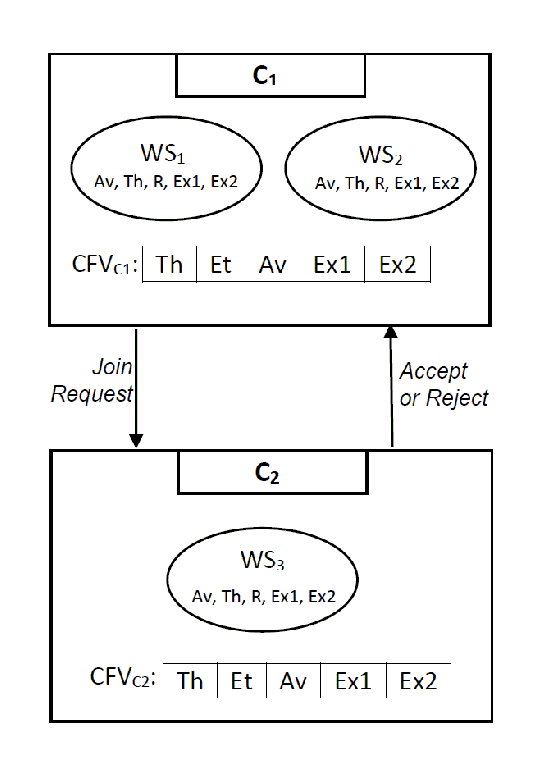
\includegraphics[width=3.25in]{figures/cfvs.eps}}
\caption{Communities with different properties of web services actively looking for other communities to collaborate with, they send collaboration requests to communities they find the collabration  increasing the gain}
\label{fig_community}
\end{figure}

Now, we want to generate a set of feature vectors representing the communities of web services for training purposes. For communities, we add two additional external features, as discussed in Section \ref{s:ef} that reflect the community's estimation of its quality metrics compared to other web services. Therefore, we formulate a \emph{Community Feature Vector (CFV)} as $CFV_{<C>} = \{f_1,...f_5\}$ having a community of $k$ web services. $C = {ws_1,...ws_k}$. The features $f_1$ through $f_5$ represent the \emph{execution time}, \emph{throughput}, \emph{availability} and the \emph{external parameters 1 and 2} correspondingly. A set of communities, with their feature vectors and utilities evaluated, provides our algorithm with a raw training data set. We call this set of communities the \emph{template vector}, and the set of feature vectors associated with the \emph{template vector} is referred to as the \emph{community feature vector set (CFVS)}. Figure \ref{fig_community} depicts communities looking to form collaborate communities and join other communities in order to improve their utility gain.

\subsubsection{Feature Engineering}\label{sss:feng}
Let $CFVS = \{C_1, C_2,..., C_N\}$ be the community feature vector set with $N$ communities. Based on the $CFVS$ set, we create an $|N \times N|$ gain matrix for $t$ different time slots. Each entry of $gain_{n,m}^{t}$corresponds to a utility gain of web services in $C_n$, when $C_n$ joins $C_m$, based on community and web service data available for time $t$. All of these values have to be evaluated by implementing the community with members of $ws_i \in C_n$ and $ws_j \in C_m$ and evaluating its utility (see Equation \ref{u_c_load}). Therefore $gain_{n,m}^{t} = U_{C_n \cup C_m}^{t} - U_{C_{n}}^{t}$. Evaluating the utility gain for all entries of the $gain$ matrix can be a costly process with a very big number of $N$, size of the feature vector $|N|$ should be chosen carefully. 

Now, we let our set of communities in the $CFVS$ set, within $|T|$ time frame iterations, choose the the best communities to join. Each community is provided with the corresponding row of data from the $gain$ matrix. Basically, $C_i$ is provided with the data in row $i$ of matrix $gain_{N,N}$, which is all of the possible utility values it can gain by joining different communities. By ordering the list, each community is utilized with an ordered set of preferences over other communities it likes to join. We define $>_{i}^t$ as the preference order of community $i$ at time $t$.

Let $P_{C_i}^t = \{C_1 >_{i}^t C_2 >_{i}^t .... >_{i}^t C_n\}$ be an ordered set of preferences for community $C_i$ at time $t$. Based on this ordered set, we define $K^t(C_i, k)$ as a set of the $k$ most preferred communities of community $i$ at time $t$.
%\subsubsection{feature vector generation}\label{sss:fvg}
\begin{equation}\label{h_t_pref_top}
\begin{split}				
K^t(C_i, k) = &\Big\{C_x | C_x >_{i}^t C_y; \forall C_y \in CFVS\ \\
				      &\wedge C_y \notin \{K^t(i, 1),K^t(i, 2),...,K^t(i, k-1)\} \Big\}				
\end{split}
\end{equation}
Based on $K^t(C_i, k)$, we define a set of communities for $C_i$ in which they are the k most preferred communities for community $i$ and also community $i$ belongs to the k most preferred communities out of all of the communities in set $K^t(C_i, k)$. This basically implies the preference is both-sided.
\begin{equation}\label{l_t_top_both}
\begin{split}	
L^t(C_i,k) = &\Big\{C_j | C_j \in K^t(C_i, k) \\
             &\wedge C_i \in \bigcup_{C_x \in K^t(C_j, k)}K^t(C_x, k)\Big\}
\end{split}
\end{equation}

Table \ref{table:nonlin} illustrates an example of a $gain$ matrix for 3 different communities and their combinations. Each row shows the gain the community can achieve by collaborating with other 5 communities. In this example for community $\textless 348 \textgreater$ we have: \\
$K(\textless 348 \textgreater, 1) = \{\textless1934, 2117\textgreater\}$ and \\
$K(\textless 348 \textgreater, 2) = \{\textless1934, 2117\textgreater, \textless1934\textgreater\}$ \\
Since $\textless 348 \textgreater$ is best preferred community of $\textless 1934, 2117 \textgreater$ therefore $L(\textless 348 \textgreater, 1)$ is not empty and contains the community $\textless1934, 2117\textgreater$.

Using the $gain$ matrix and the mentioned preference ordering relations, we are able to build a decision tree where the list of possible communities to join and their expected utilities are set.
% as well as the joined events that took place in different time slots. 
In addition to best choices, web services have access to other ordered choices and can look for the second best or third best if their first try is rejected by the target community. The consequences of each try level is analyzed in more detail in the following section, in which we launch experiments and investigate the effectiveness of the use of a decision tree with different decision layers in joining other communities and enhancing the overall utility. 

\subsection{Decision Profile Generation}\label{ss:learningmodel}

Our goal is to create a decision making profile for each community in the $CFVS$ set. We are creating an environment where they can experience the outcomes of different strategies. The result will be a decision tree of the feasible and utility increasing moves over time.

We let communities pick the best communities for maximizing their utilities over different time frames. At time $t = 1$, we let each community in the $CFVS$ set choose the best community, which is a single community in set $C_j = K^t(C_i, 1)$. If community $C_j$ also has the highest preference to join $C_i$ meaning the $L^t(C_i, k=1)$ set is not empty, they would join together. Having set $k = 1$ is a very strict and hardly satisfiable condition. In order to relax the requirement, the value of $k$ is being increased by a rate $r$ proportional to time slot $t$. Basically, $k = 1 + |r \times t|$. On early steps of simulation web services and communities are more strict but as time goes on, we let them choose second and then third best options too. However, increasing $k$ quickly increases the time complexity of $K^t(C_i, k)$ by $O(k^2 \times n.log(n))$. 

When communities $C_i$ and $C_j$ are in each other's top $k$ preference set, their combination is added to the list of possible communities that can join others at time $t+1$. Also, for each community $C_i$ in our initial $CFVS$ set, we maintain a tree with the community $C_i$ as its root. Its children are all of the communities that $C_i$ decided to join. As the scenario progresses over time, the merged communities may decide to join other communities. When community $C_i$ and $C_j$ decide to join each other and create community $C_k$, the new community $C_k$ will be added as a child to both $C_i$ and $C_j$ nodes. At the end of the process, each community is utilized with a tree of set of possible combination of communities it can join. Algorithm \ref{algo:dectree} illustrates the DDM tree creation procedure as pseudo-code.

Having created $|n|$ trees, for each community $C_i$, our communities are utilized with the different possible paths they can take to maximize their utilities. Using a distance function, communities and web services can utilize these results and find the $C_i$ that closely resembles their parameters. They will be utilized with a tree that has the strategies the community can use to join our communities which will be best possible path to take and communities to join while most likely being accepted by other communities since its a two sided preference. The algorithm below describes the tree creation process.

\begin{algorithm}
\DontPrintSemicolon
\KwIn{$\langle r, gain^t_{n,n}, CFVS \rangle$ learning rate $r$, $|N \times N \times T|$ gain matrix, community feature vector}
\KwOut{A set of \emph{root} nodes of the decision trees}
$k \gets 1$\;
$nodes[N] \gets$ initialize $N$ tree nodes representing each community in CFVS\;
\For{$t \gets 1$ \textbf{to} $T$} {
	$k \gets 1 + round (r \times t)$\;
  \For{all $C_i \in CFVS$} {
	  \For{all $C_j \in L^t(C_i, k)$} {
      % The "l" before the If makes it so it does not expand to a second line
      \If{$C_i \in L^t(C_j, k)$}{
        $C_k \gets C_i \cup C_j$\;
				add $C_k$ to $CFVS$ set\;
				initiate $node_k$, representing $C_k$\;
				$nodes_i.addChild (node_k)$\;
				$nodes_j.addChild (node_k)$\;
      }
%      \Else{
%        $j \gets j + 1$\;
%      }			
		}
  }
%  $i \gets i + 1$\;
}
\Return{nodes}\;
\caption{{\sc DDM Decision Tree Algorithm}}
\label{algo:dectree}
\end{algorithm}

\textbf{Complexity.} Here we analyze the computational complexity of the DDM decision tree creation algorithm on each time iteration $t$. Computing top $k$ preferred communities for $C_i$ in $L^t(C_i, k)$ requires an $O(n.log(n))$ sort time. $C_i$ has a result set of size $|k|$, and for each of those $k$ communities we need to check against their $k$ top preferred communities. Considering we already have the list sorted, line 6 in algorithm runs $O(k \times n.log(n))$ times. Doing this search for all communities in $|CFVS|$ set $n$ times (line 5), the overall order of complexity of the algorithm in regards with $n$ and $k$ is: $O(k^2 \times n^2.log(n))$.

\section{Experiments}\label{s:experiments}
We implemented DDM in Java\footnote{Source code of implementation and data is available at: \emph{https://github.com/Marooned202/DDM}}. We have extracted the set of features for 4532 web services in 64 different time slots through a data set provided by \cite{10.1109/ISSRE.2011.17}. By choosing 86 web services out of these sets and choosing a subset of all possible combinations of sizes 2, 3, and 4 of these 86 web services, we have chosen 10,000 communities and evaluated the feature vectors and utilities they can have in 64 different time slots. This provides us with the initial training feature set of size $|CFVS| = 10,000$ communities. Based on Equation \ref{u_c_load} the utility of these communities are estimated, and the gain matrix $|10000 \times~ 10000|$ of all possible ways of merging these 10,000 communities, is generated\footnote {The template vector and gain matrix generated are available at \emph{https://github.com/Marooned202/DDM/tree/master/wsds/data/run}}, and each community has the ordered preference among other communities known in the set. 

We let communities and web services adopt their strategies based on our $DDM$ decision making mechanism. Based on the decisions adopted, each community will generate a decision tree profile. We let DDM run four times with different $r$ rates of 0.05, 0.07, 0.10 and 0.20. With the slow rate of $r = 0.05$, we increase $k$ in Equation \ref{u_c_normal} for every 20 time frames, which will happen only three times in our 64-step experiment. In the case of $r = 0.20$, k increases much faster, at a rate of once every 5 time frames, which increases the complexity of the $L^t(C_i,k)$ search for each community in the $CFVS$ set. 

Table \ref{table:valueandgain} depicts the average utility gain value of the communities in each of the four runs. The utility gain is the increase of utility the communities gain by cooperating and joining other communities. The utility gain ratio is the ratio of their final utility over initial utility. Comparing the different search rates, we can see increasing $r$ to value of $0.10$ results in significant performance boost, however the higher rates of $r$ are not increasing the chance of finding better collaborative groups for our communities. 

\begin{table}[ht]
\caption{Utility gain of web services after making collaborative groups based on DDM algorithm with different $r$ rates} % title of Table
\centering % used for centering table
{\renewcommand{\arraystretch}{1.2}
\begin{tabular}{c|c|c} % centered columns (4 columns)
\hline\hline %inserts double horizontal lines
Search Rate $r$ & Utility Gain Value & Utility Gain Ratio \\ [0.5ex] % inserts table
%heading
\hline % inserts single horizontal line
r=0.20 & 176.1499 & 6.9690 \\
r=0.10 & 174.6541 & 6.9182 \\
r=0.07 & 159.9462 & 6.2834 \\
r=0.05 & 136.0768 & 5.1032 \\ [1ex] % [1ex] adds vertical space
\hline %inserts single line
\end{tabular}
}
\label{table:valueandgain} % is used to refer this table in the text
\end{table}


%\begin{figure}%[!t]
%\centering
%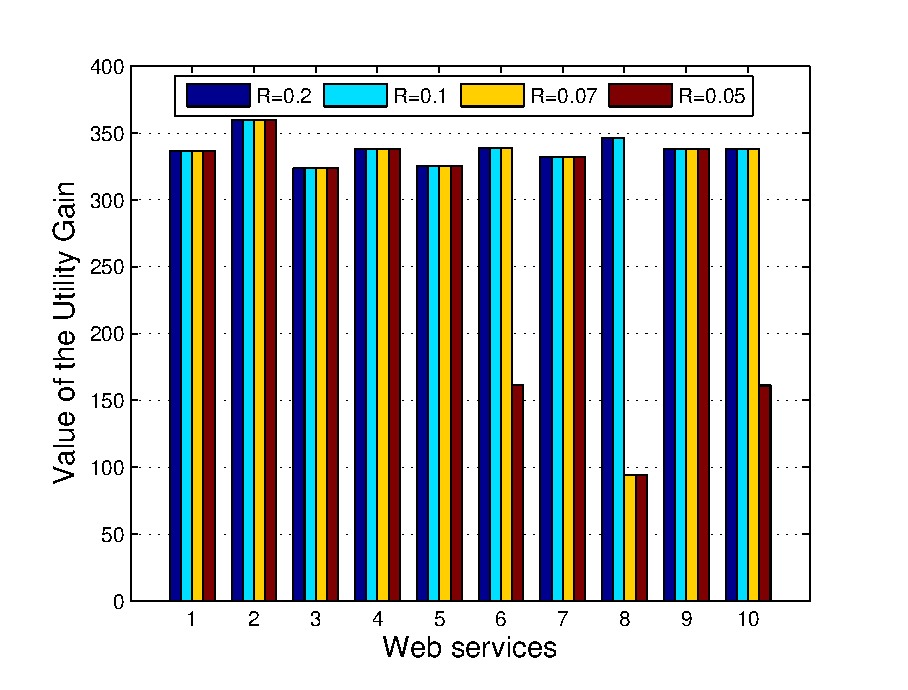
\includegraphics[width=3.5in]{figures/utility_gain_r.eps}
%\caption{DDM Utility Gain Value}
%\label{utility_gain_value}
%\end{figure}
%
%\begin{figure}%[!t]
%\centering
%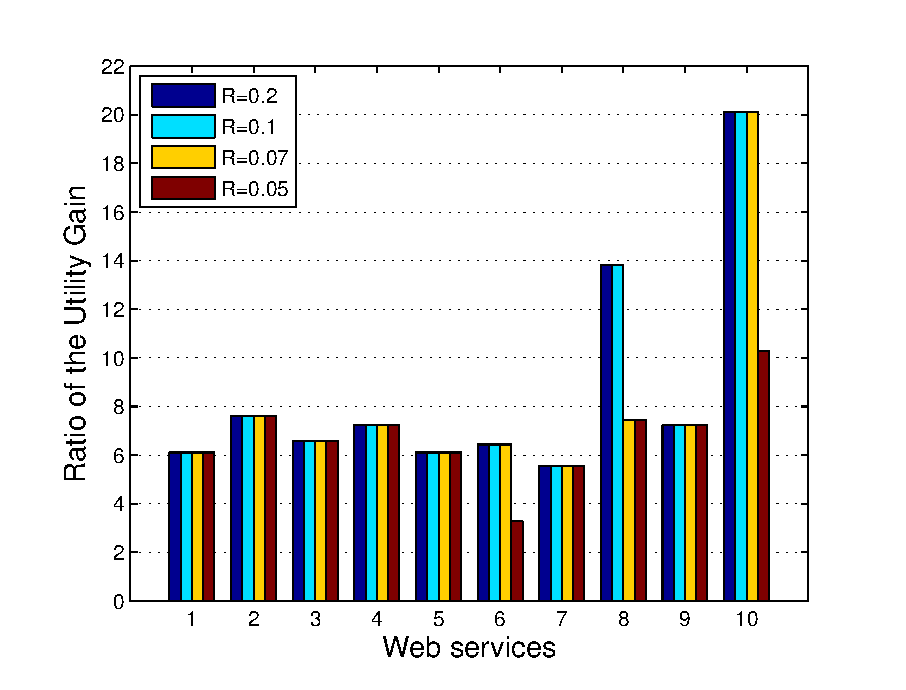
\includegraphics[width=3.5in]{figures/utility_ratio_r.eps}
%\caption{DDM Utility Gain Ratio}
%\label{utility_gain_ratio}
%\end{figure}

We utilize the same communities and web services with a simple rational decision making mechanism, in which communities will choose to join a community if it increases utility by any amount. We call it the $rational$ method, in the sense that it is just a rational method and is not aiming to be optimal. We chose 10 random web services and compared the results with web services which adopted our DDM model. Figure \ref{utility_gain_mlisa_and_rational} shows the comparison of the end result of utility gain values. In 18 out of 40 tries, \emph{rational} agents were not able to improve their utility at all because the communities they chose rejected their request, most likely because they would not have increased the utility of the other communities if they had joined them. The results show that a long-term strategic decision mechanism is needed to satisfy all of the services within communities. Figure \ref{utility_gain_mlisa_and_rational_ratio} shows the same results in terms of ratio of utility gain.

\begin{figure}%[!t]
\centering
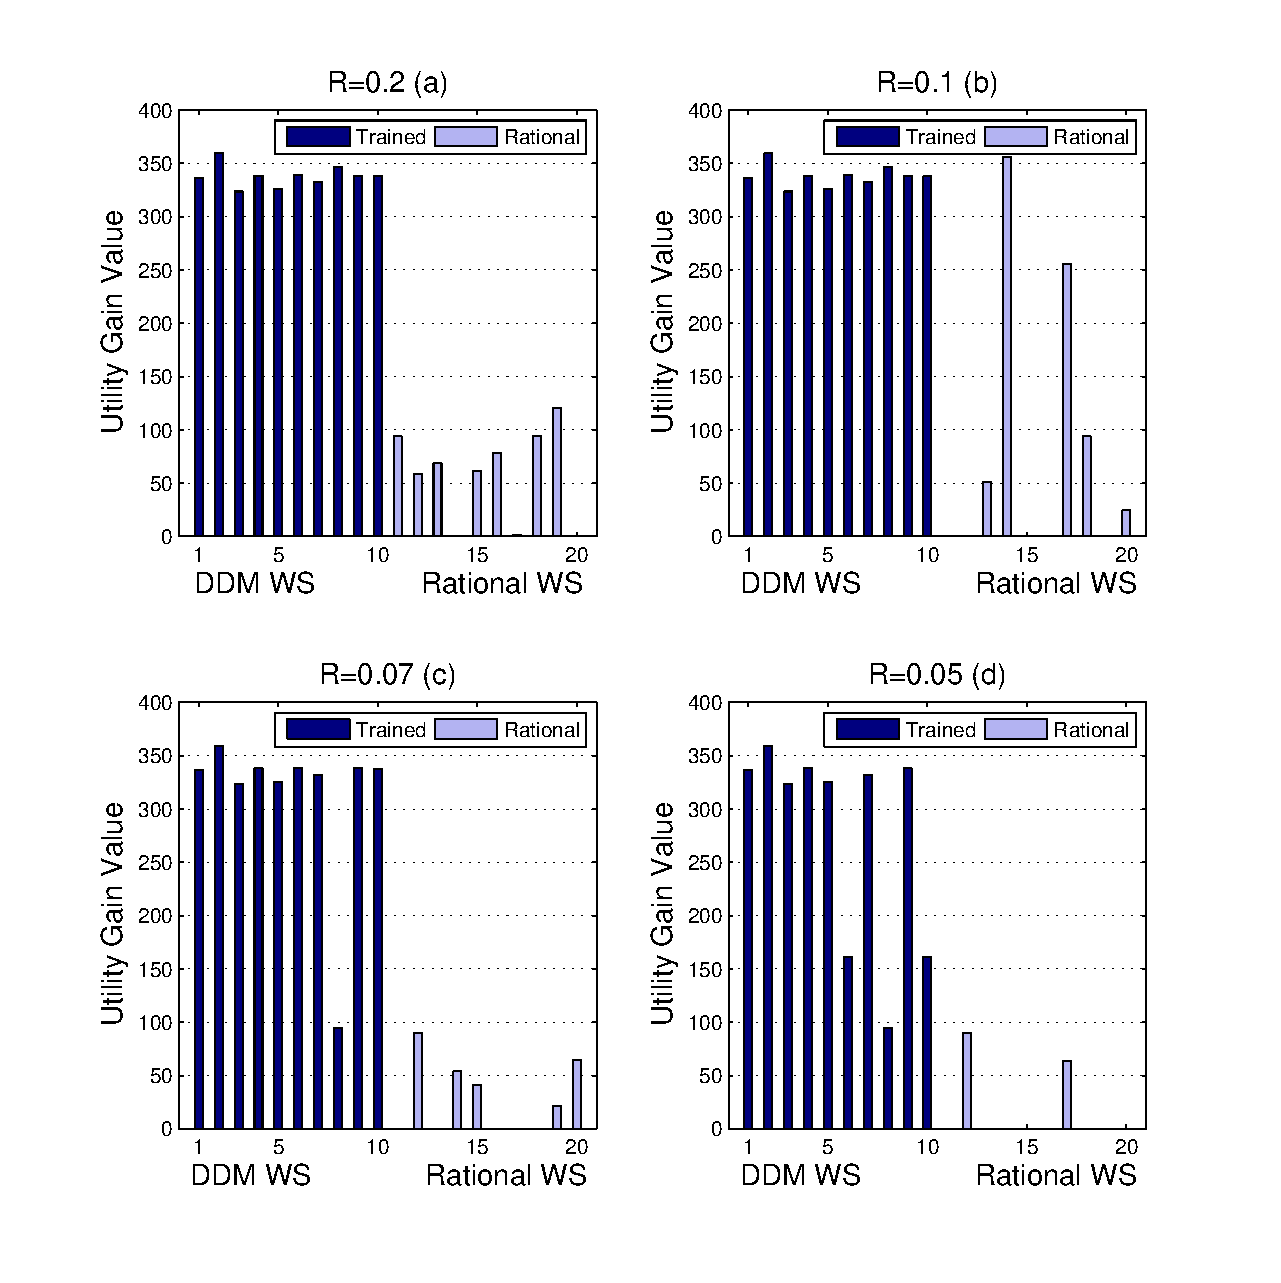
\includegraphics[width=3.5in]{figures/utility_gain.eps}
\caption{Utility Gain DDM and Rational}
\label{utility_gain_mlisa_and_rational}
\end{figure}

\begin{figure}%[!t]
\centering
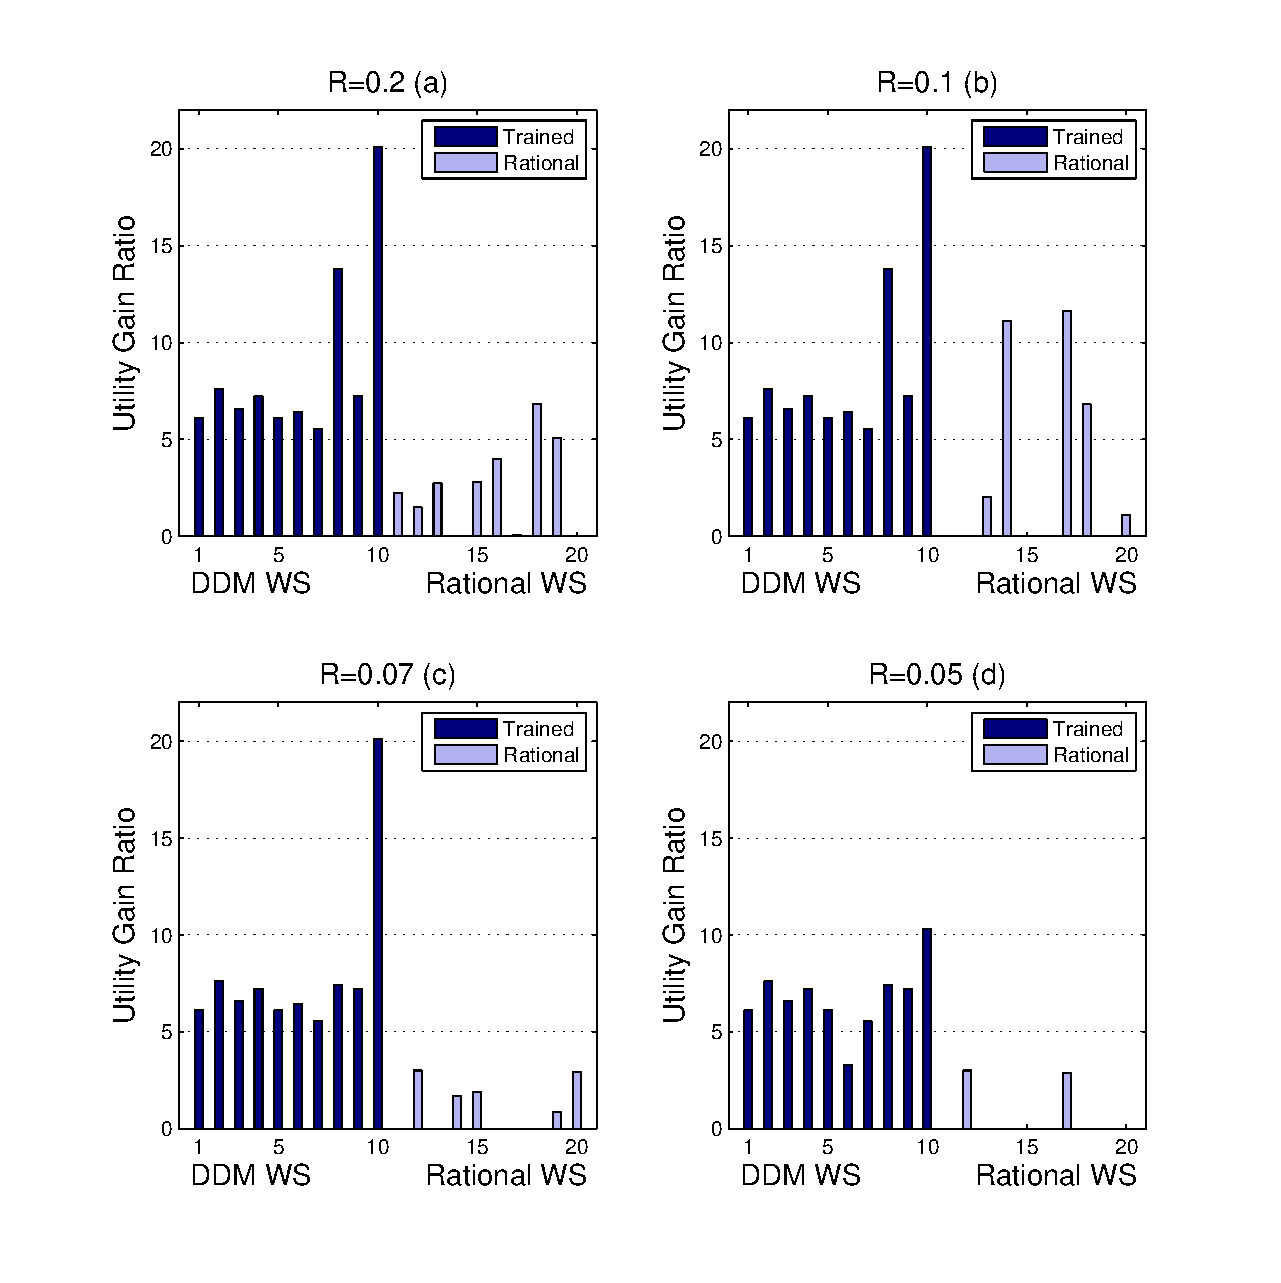
\includegraphics[width=3.5in]{figures/utility_ratio.eps}
\caption{Ratio of Utility Gain DDM and Rational}
\label{utility_gain_mlisa_and_rational_ratio}
\end{figure}

Now, we evaluate the performance of the decision profiles generated based on our data set for other communities.% which are not included in the decision tree creation process. 
We create one thousand communities from the web services in the data set that were not involved in the decision model creation process. We define a distance function that measures the difference between basic features of communities, which measures the similarity of communities.

\begin{equation}\label{distance_c}
\begin{split}
distance (C_1, C_2) & = |Th_{C_1} - Th_{C_2}| \\
                    & + |A_{C_1} - A_{C_2}| + |Et_{C_1} - Et_{C_2}|
\end{split}
\end{equation}

Now, each community tries to find the closest community within the trained $CFVS$ set. Following its decision profile, the community can get a good estimate of the possible strategic decisions it can adopt. Basically, the trained profiles benefit the new web services in two ways. First, they provide the communities with a set of viable communities to join. Second, they provide an estimation of long-term utility gain for each available decision. In this experiment, we let communities follow the best decision within the decision tree provided to the them. 

\begin{table}[ht]
\caption{Number of communities that misses the optimal decision, out of 1,000 communities} % title of Table
\centering % used for centering table
\begin{tabular}{|c|c|} % centered columns (4 columns)
\hline %inserts double horizontal lines
 Method&Miss \\ [0.5ex] % inserts table
%heading
\hline % inserts single horizontal line
 DDM r=0.05& 375 \\ % inserting body of the table
 DDM r=0.07& 137 \\
 DDM r=0.10& 6 \\
 DDM r=0.20& 6 \\
Rational Method& 717 \\
Greedy Method& 828 \\ [1ex] % [1ex] adds vertical space
\hline %inserts single line
\end{tabular}
\label{fail_rate} % is used to refer this table in the text
\end{table}


In order to evaluate the performance of the mechanism, we used \emph{Receiver Operating Characteristic (ROC) curve}, which is a graphical plot illustrating the true negative rate against the false positive rate at various threshold settings in classifier systems. In order to classify our communities' selection strategies correctly, for each community, we evaluated the training process by replacing the community in the set with the closest one, from which it gets the strategy profile. If the actions are the same and the same utility levels are gained, we classify the decision as correct. Otherwise, it is classified as a wrong decision. \emph{AUC}, the area under the \emph{ROC curve}, is equal to the probability that a classifier will rank a randomly chosen positive instance higher than a randomly chosen negative one, and the higher number reflects better performance from the better solution.  Figure \ref{roc5} illustrates the \emph{ROC curve} evaluation of the DDM decision making mechanism. We compare our method with two other methods. The \emph{rational} method is based on the assumption that communities, as rational agents, join a community that increases their utility. The \emph{greedy} method only looks up the available list of communities and simply joins the community that maximizes its utility without considering any long-term strategy or other communities' acceptance scenarios, its an greedy algorithm and chooses a locally optimal choice. Therefore we use these two methods as our benchmark:

\begin{itemize}
  \item {\bf Rational Method:} Communities would send a join request to any available community, which will increase the utility. The other community would accept the join offer if the utility gain is positive as well.
	\item {\bf Greedy Method:} Communities do a linear search among all the available communities and send a join request to the community which results in maximum utility, The other community would accept the join offer if the utility gain is positive and the utility gain does not need to be the maximum for the community recieving the join request.
\end{itemize}

Figure \ref{roc5} compares the results for all methods. The two other methods have very high failure rates compared to our method. Table \ref{fail_rate} illustrates the number of communities that failed to find the optimal collaboration group. The results support the need for a long-term training model in a successful decision making process.

\begin{figure}%[!t]
\centering
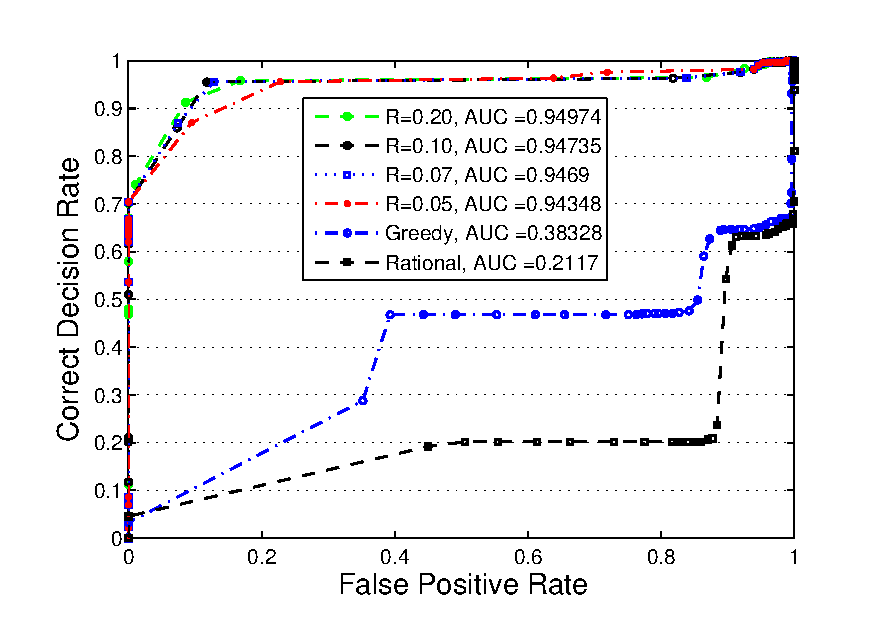
\includegraphics[width=3.5in]{figures/roc.eps}
\caption{RoC Curve}
\label{roc5}
\end{figure}
Now, we evaluate the system-specific results from users' and communities' perspectives. By distributing tasks among the communities over these time frames, we evaluate the revenue for each community. Figure \ref{stats1} shows the overall revenue gain of communities using our method. Figure \ref{stats2} shows the momentarily revenue gain for each community in each time slot compared to the previous time. These results show that the run with the higher learning rate of $r=0.20$ starts discovering better communities to join much earlier. The runs with slow rates seem to find some communities to join initially, but then they slow down until later, when they start discovering new communities to join.

\begin{figure}%[!t]
\centering
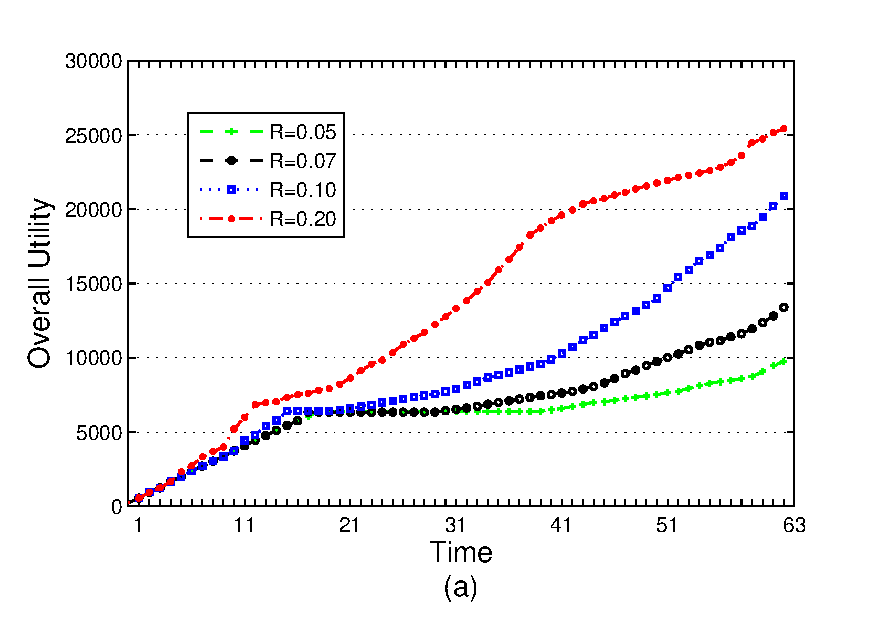
\includegraphics[width=3.5in]{figures/stats1.eps}
\caption{Overall Utility of all communities}
\label{stats1}
\end{figure}


\begin{figure}%[!t]
\centering
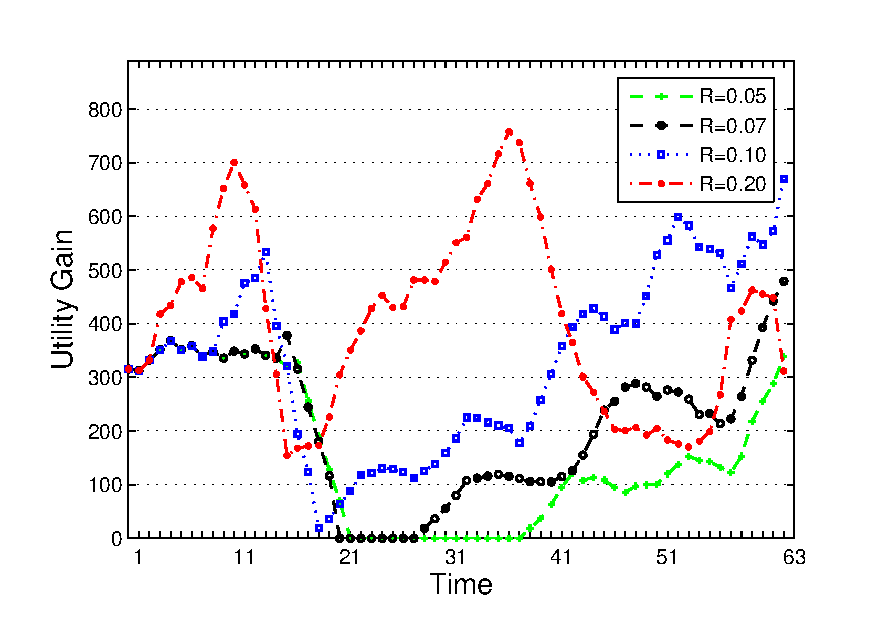
\includegraphics[width=3.5in]{figures/stats2.eps}
\caption{Utility Gain on time}
\label{stats2}
\end{figure}

Figure \ref{stats3} depicts the average community size over time, which essentially represents the number of new communities being formed. Once again, these results show that the runs with higher search rates tend to find appropriate communities to join faster.

\begin{figure}%[!t]
\centering
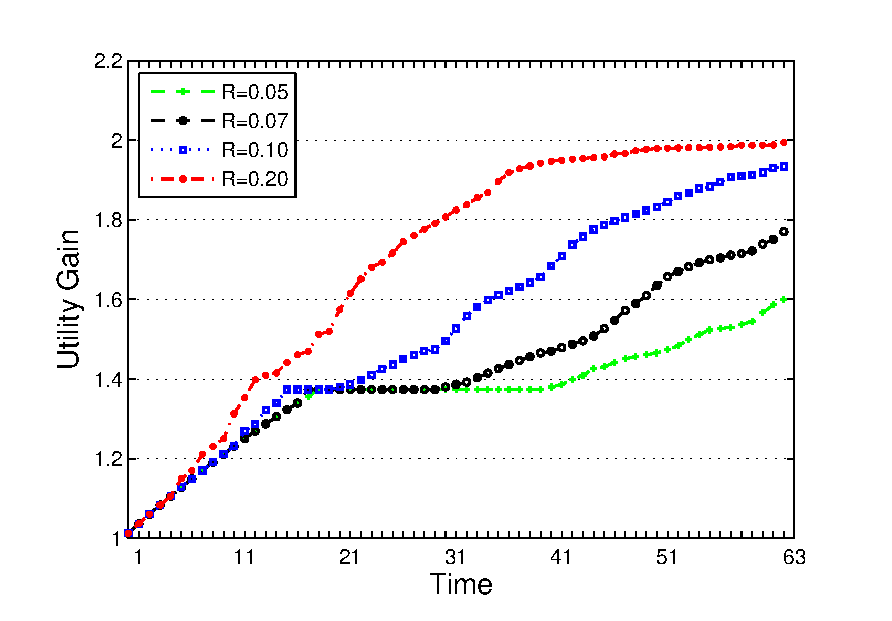
\includegraphics[width=3.5in]{figures/stats3.eps}
\caption{Average Community Size}
\label{stats3}
\end{figure}

\section{Related Work}\label{s:related_work}

In \cite{DBLP:journals/internet/BenatallahSD03}, Benatallah et al.
defined communities as \emph{Service Containers} that aggregate
substitutable web services providing a common functionality (same
set of operations). They abstracted \emph{Service Containers} as
web services that are created, advertised, discovered and invoked
just as elementary web services. The \emph{Container} is
considered as a manager that is responsible for web service
selection upon receiving a request on run-time. The authors have
proposed a scoring service based on non-functional requirements of
the request and web service capabilities to dynamically chose the
web service to perform the requested task. A similar concept was
proposed by Maamar et al. in
\cite{DBLP:journals/ijebr/MaamarSTBB09}. The authors introduced
web service communities as a collection of web services with a
common functionality but different QoS properties. A community
manager, upon receiving a request, delegates the request to one of
its current members. The choice is based on the performance
history and quality metrics of each web service. The authors have
proposed an efficient global web service selection algorithm in
order to approach quality constraints and preferences for
composite services which require aggregation of different types of
services to satisfy the user.

Benslimane et al. \cite{Liris-2770} have proposed a multi-layer
approach grouping similar Web services into communities and having
an interface implemented as an abstract web service for accessing
the community on top of the community layer. The interactions
between composite, management and community layers and the
bindings are performed by a generic driver called Open Software
Connectivity (OSC).

In \cite{managing-hela-jalel}, Limam and Akaichi have proposed web
service communities with centralized access across distributed web
services. They have proposed a framework for web service
management, query resolution among communities and a query caching
mechanism executed by the manager to improve the performance of
query resolution process among many distributed communities. The
key idea is to cache previous computed results for answering
future queries.


Maamar et al. initially in \cite{conf/webist/MaamarLBTS07} and
then comprehensively in \cite{DBLP:journals/ijebr/MaamarSTBB09}
proposed an architecture utilizing \emph{Contract-Net} protocol
for engineering task distribution within communities of web
services. The protocol is centrally executed by the community
manager. This architecture has been further developed in
\cite{CSTintercommunity, conf/IEEEscc/BenharrefSBB11,
conf/IEEEscc/KhosravifarBMMT10, conf/aina/LimTM11}. Two types of
roles have been distinguished for community members: masters and
slaves. Master web services and community managers that lead
communities and are responsible for membership management. They
can invite and convince slave web services to join the community,
and attract new slave web services to their communities by
awarding them better payoff. Moreover, they can eject some slave
members from the community to improve its overall reputation if
these members are misbehaving or cannot provide the promised QoS.

In \cite{Medjahed05adynamic}, Medjahed and Bouguettaya have
developed a community as a ``cluster'' that groups Web services
based on a specific area of interest. All web services in a given
community share the same functionality. These communities are
created by \emph{third party community providers} which use the
\emph{community ontology} as a template and define a set of
operations that all web services within a community should
provide. Using semantic analysis on web service operations, web
services either find and join a community with similar
functionality or create a new operation description for a new
community. The authors have described the concept of
\emph{community agents} associated to \emph{community providers}.
A community agent is responsible, among other things, of the
registration of services with the community. An example of a
community that provides health care services to senior citizens
has been used. In this example, a governmental entity is needed to
check the health care standards used by the members before
authorizing them to be part of the community. Such a central
entity is represented by the community agent. Thus, community
agents are playing the role of community managers. In a close work
\cite{Zeng:2003:QDW:775152.775211}, Zeng et al. have described a
global planning selection algorithm and a delegation algorithm to
be run when a request to execute an operation is received by the
community. This needs a central entity to run those algorithms.
Such entity plays the same role as the community coordinator or
manager.

Most of the recent work on communities of services are either
user-centric and focus on user satisfaction
\cite{Chun02user-centricperformance} or system-centric and focus
on the whole system throughput, performance and utilization. There
are many contributions in distributed, grid, cluster and cloud
services which are system-centric. However, in real world
environments and applications, both users and service providers
are self-interested agents, aiming to maximize their own profit.
In those environments, both parties (users and services) will
collaborate as long as they are getting more benefits and payoff.

In this direction, recently \cite{DBLP:conf/IEEEscc/LimTMB12,
DBLP:conf/IEEEscc/KhosravifarABT11, 10.1109/TSC.2012.12} proposed
mechanisms to help users and services maximize their gain. A
two-player non-cooperative game between web services and community
master was introduced in
\cite{DBLP:conf/IEEEscc/KhosravifarABT11}. In this game-theoretic
model, the strategies available to a web service when facing a new
community are requesting to join the community, accepting the
master's invitation to join the community, or refusing the
invitation to join. The set of strategies for communities are
inviting the web service or refusing the web service's join
request. Based on their capacity, market share and reputation, the
two players have different sets of utilities over the strategy
profiles of the game. The main limits of this game model are: 1)
its consideration of only three quality parameters, while the
other factors are simply ignored; and 2) the non-consideration of
the web services already residing within the community. The game
is only between the community master and the new web service, and
the inputs from all the other members and their influence on the
master's decision are simply ignored. The consideration of those
inputs and this influence factor is a significant issue as
existing web services can lose utility or payoff because of the
new member, which can result in an unhealthy and unstable group.
The problem comes from the fact that the existing members should
collaborate with the new web services, so probably their
performance as a group can suffer. Existing members may even
deviate and try to join other communities if they are unsatisfied.
Those considerations of forming stable and efficient coalitions
are the main contributions of our paper.

In \cite{DBLP:conf/IEEEscc/LimTMB12}, a 3-way satisfaction approach
for selecting web services has been proposed. In this approach,
the authors proposed a web service selection process that the
community masters can use. The approach considers the efficiency
of all the three involved parties, namely users, web services and
communities. In this work, it is shown how the gains of these
parties are coupled together using a linear optimization process.
However, the optimization problem in this solution tends to
optimize some parameters considering all web services regardless
of their efficiency and contribution to the community's welfare.
Moreover, there are no clear thresholds for accepting or rejecting
new web services. The solution of the optimization problem could,
for instance, suggest web services already residing within the
community to increase or decrease their capacity to cover up the
weakness of other parties in the system. However, a high
performing web service could deviate anytime it finds itself
unsatisfied within the community instead of adjusting its service
parameters.

In \cite{10.1109/TSC.2012.12}, a cooperative scheme among
autonomous web services based on coalitional game theory has been
introduced. The authors have proposed an interesting algorithm to
reach individually stable coalition partition for web services in
order to maximize their efficiency. The communities choose new web
services on the promise that it would benefit the community
without decreasing any other web service's income. In the proposed
model, the worth of community is evaluated with high emphasis on
the availability metric and considering price and cost values
only. The community structure is based on a coordination chain,
where a web service is considered as a \emph{primary} web service
and the community task-distribution method initially invokes the
primary web service and only if the primary web service is
unavailable, the method invokes the next backup web services as
they are ordered in the coordination chain. We believe that this
coordination chain limits the cooperation power as it introduces a
sort of hierarchy. However, in pure and open cooperative models,
such as the one we propose in this paper, active cooperation
activities engaging simultaneously many agents so that they can
perform the tasks more efficiently are being used. Moreover, if
the availability is high, which is the case nowadays with the
recent advancements in cloud and hardware infrastructures, the
backup web services will end-up having a very low chance of
getting jobs, especially the ones further in the chain. This will
results in a considerable waste of web services capabilities.

All the proposed frameworks share a common aspect, which is providing the solution based on assumption of having complete information of all services and performing evaluations based on a large number of input each time they want to adopt a strategic decision making process. 
So basically These solutions generally suffer from high complexity, which makes decision making impossible in an on-demand fashion, or they simplify important aspects to make it practical in the real world, thereby hurting the decision making performance. We address this issue by introducing DDM a framework that operates based on a trained model that regulates web service agents' decision making process in terms of cooperating with one another. After being trained, web services get to compute expectations as utilities they would gain while cooperating with communities of different characteristics. Therefore web services and communities can make prudent decisions when inviting a web service to join or accepting a join inquiry initiated from a web service. In general, DDM equips web services with efficient methods for foreseeing how their choices will impact their long-term and short-term goals; therefore, opting for best decision available. 

%\subsection{Subsection Heading Here}
%Subsection text here.

% needed in second column of first page if using \IEEEpubid
%\IEEEpubidadjcol

%\subsubsection{Subsubsection Heading Here}
%Subsubsection text here.Subsubsection text here.Subsubsection text here.Subsubsection text here.Subsubsection text here.Subsubsection text here.Subsubsection text here.Subsubsection %text here.Subsubsection text here.Subsubsection text here.Subsubsection text here.Subsubsection text here.Subsubsection text here.
%Subsubsection text here.Subsubsection text here.Subsubsection text here.

%Subsubsection text here.Subsubsection text here.Subsubsection text here.Subsubsection text here.Subsubsection text here.Subsubsection text here.Subsubsection text here.Subsubsection %text here.Subsubsection text here.Subsubsection text here.Subsubsection text here.Subsubsection text here.Subsubsection text here.Subsubsection text here.


% An example of a floating figure using the graphicx package.
% Note that \label must occur AFTER (or within) \caption.
% For figures, \caption should occur after the \includegraphics.
% Note that IEEEtran v1.7 and later has special internal code that
% is designed to preserve the operation of \label within \caption
% even when the captionsoff option is in effect. However, because
% of issues like this, it may be the safest practice to put all your
% \label just after \caption rather than within \caption{}.
%
% Reminder: the "draftcls" or "draftclsnofoot", not "draft", class
% option should be used if it is desired that the figures are to be
% displayed while in draft mode.
%
%\begin{figure}[!t]
%\centering
%\includegraphics[width=2.5in]{myfigure}
% where an .eps filename suffix will be assumed under latex,
% and a .pdf suffix will be assumed for pdflatex; or what has been declared
% via \DeclareGraphicsExtensions.
%\caption{Simulation Results}
%\label{fig_sim}
%\end{figure}

% Note that IEEE CS typically puts floats only at the top, even when this
% results in a large percentage of a column being occupied by floats.
% However, the Computer Society has been known to put floats at the bottom.


% An example of a double column floating figure using two subfigures.
% (The subfig.sty package must be loaded for this to work.)
% The subfigure \label commands are set within each subfloat command, the
% \label for the overall figure must come after \caption.
% \hfil must be used as a separator to get equal spacing.
% The subfigure.sty package works much the same way, except \subfigure is
% used instead of \subfloat.
%
%\begin{figure*}[!t]
%\centerline{\subfloat[Case I]\includegraphics[width=2.5in]{subfigcase1}%
%\label{fig_first_case}}
%\hfil
%\subfloat[Case II]{\includegraphics[width=2.5in]{subfigcase2}%
%\label{fig_second_case}}}
%\caption{Simulation results}
%\label{fig_sim}
%\end{figure*}
%
% Note that often IEEE CS papers with subfigures do not employ subfigure
% captions (using the optional argument to \subfloat), but instead will
% reference/describe all of them (a), (b), etc., within the main caption.


% An example of a floating table. Note that, for IEEE style tables, the
% \caption command should come BEFORE the table. Table text will default to
% \footnotesize as IEEE normally uses this smaller font for tables.
% The \label must come after \caption as always.
%
%\begin{table}[!t]
%% increase table row spacing, adjust to taste
%\renewcommand{\arraystretch}{1.3}
% if using array.sty, it might be a good idea to tweak the value of
% \extrarowheight as needed to properly center the text within the cells
%\caption{An Example of a Table}
%\label{table_example}
%\centering
%% Some packages, such as MDW tools, offer better commands for making tables
%% than the plain LaTeX2e tabular which is used here.
%\begin{tabular}{|c||c|}
%\hline
%One & Two\\
%\hline
%Three & Four\\
%\hline
%\end{tabular}
%\end{table}


% Note that IEEE does not put floats in the very first column - or typically
% anywhere on the first page for that matter. Also, in-text middle ("here")
% positioning is not used. Most IEEE journals use top floats exclusively.
% However, Computer Society journals sometimes do use bottom floats - bear
% this in mind when choosing appropriate optional arguments for the
% figure/table environments.
% Note that, LaTeX2e, unlike IEEE journals, places footnotes above bottom
% floats. This can be corrected via the \fnbelowfloat command of the
% stfloats package.



\section{Conclusion}\label{s:conclusion}

In this paper, we proposed a training model for the problem of membership management of communities of web services. Using the traning model we created a decision making profile for each community and web service involved which provides them with a set of feasible and utility increasing moves. This utilized our web services with efficient methods of foreseeing how their choices of actions would impact their long-term and short-term goals, therefore they opted for best decision available. The ultimate goal is to choose the best decision when it comes to communities formation, among many possible short-term rational and utility increasing choices. The experimental results show that our algorithms provide web services and community owners, in real-world-like environments, with applicable and near-perfect decision making mechanisms. The results of experiments using real data samples support the need for a long-term training model in a successful decision making process.

Our plan for future work is to advance learning process on the training set that we provided in our work. SVN machine learning algorithm are suitable in classification of our training data set, to better classify correct or wrong decisions based on long-term utility gains, as data set outputs. This can further facilitate the process of finding optimal cooperators in regards to enhancing web services' overall performance as service providers.

%% The Appendices part is started with the command \appendix;
%% appendix sections are then done as normal sections
%% \appendix

%% \section{}
%% \label{}

%% If you have bibdatabase file and want bibtex to generate the
%% bibitems, please use
%%
\bibliographystyle{elsarticle-num} 
\bibliography{Ehsan}

%% else use the following coding to input the bibitems directly in the
%% TeX file.

\begin{thebibliography}{00}

%% \bibitem{label}
%% Text of bibliographic item

%\bibitem{}

\end{thebibliography}
\end{document}
\endinput
%%
%% End of file `elsarticle-template-num.tex'.
